% Practice Test 15 — Virginia Edition
% Questions: 30 (20 MC + 10 SA)
% Generated by scripts/generate_practice_tests.py

\begin{practiceQuestion}{1-4-q07}{mc}
\begin{questionText}
The equation $y = 4.5x$ describes a proportional relationship. What is $x$ when $y = 27$?
\end{questionText}
\choiceA{$4$}
\choiceB{$5$}
\choiceC{$6$}
\choiceD{$22.5$}
\correctAnswer{C}
\explanation{$27 = 4.5x$, so $x = 27 \div 4.5 = 6$.}
\end{practiceQuestion}

\begin{practiceQuestion}{2-1-q03}{mc}
\begin{questionText}
$45$ is $75\%$ of what number?
\end{questionText}
\choiceA{$33.75$}
\choiceB{$50$}
\choiceC{$56$}
\choiceD{$60$}
\correctAnswer{D}
\explanation{Divide the part by the percent: $45 \div 0.75 = 60$.}
\end{practiceQuestion}

\begin{practiceQuestion}{2-2-q18}{mc}
\begin{questionText}
A classroom has $28$ students. $7$ of them wear glasses. What percent wear glasses?
\end{questionText}
\choiceA{$20\%$}
\choiceB{$25\%$}
\choiceC{$28\%$}
\choiceD{$35\%$}
\correctAnswer{B}
\explanation{$\frac{7}{28} = \frac{p}{100}$. Cross-multiply: $28p = 700$. Divide: $p = 25\%$.}
\end{practiceQuestion}

\begin{practiceQuestion}{2-3-q18}{mc}
\begin{questionText}
A bakery sold $160$ cupcakes on Monday and $200$ cupcakes on Tuesday. What is the percent increase from Monday to Tuesday?


\numberLine[5]{160}{205}
\end{questionText}
\choiceA{$20\%$}
\choiceB{$25\%$}
\choiceC{$30\%$}
\choiceD{$40\%$}
\correctAnswer{B}
\explanation{Change: $200 - 160 = 40$. Percent increase: $40 \div 160 = 0.25 = 25\%$.}
\end{practiceQuestion}

\begin{practiceQuestion}{2-7-q24}{sa}
\begin{questionText}
You guessed there were $300$ people at a concert. The actual attendance was $350$. Find the percent error (rounded to the nearest tenth).
\end{questionText}
\correctAnswer{$\approx 14.3\%$}
\explanation{$\frac{|300 - 350|}{350} \times 100 = \frac{50}{350} \times 100 \approx 14.3\%$.}
\end{practiceQuestion}

\begin{practiceQuestion}{3-2-q15}{mc}
\begin{questionText}
What is $(-25) + 13 + (-8)$?
\end{questionText}
\choiceA{$-20$}
\choiceB{$-46$}
\choiceC{$30$}
\choiceD{$-4$}
\correctAnswer{A}
\explanation{$(-25) + 13 = -12$. Then $(-12) + (-8) = -20$.}
\end{practiceQuestion}

\begin{practiceQuestion}{3-3-q24}{sa}
\begin{questionText}
Evaluate: $15 - 22 - (-4)$.
\end{questionText}
\correctAnswer{$-3$}
\explanation{$15 - 22 = 15 + (-22) = -7$. Then $-7 - (-4) = -7 + 4 = -3$.}
\end{practiceQuestion}

\begin{practiceQuestion}{3-4-q20}{sa}
\begin{questionText}
What is $-4.7 - 2.3$?
\end{questionText}
\correctAnswer{$-7.0$ or $-7$}
\explanation{$-4.7 + (-2.3) = -7.0$. Same signs: $4.7 + 2.3 = 7.0$, keep negative.}
\end{practiceQuestion}

\begin{practiceQuestion}{4-3-q28}{gmc}
\begin{questionText}
Three friends each receive the same gift bag containing $x$ stickers and $4$ erasers. The diagram below represents the total items.

\begin{center}
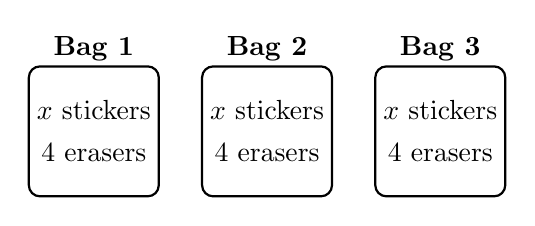
\begin{tikzpicture}[scale=0.55]
  % Bag 1
  \draw[thick, rounded corners] (0,0) rectangle (3,3);
  \node[font=\bfseries] at (1.5,3.4) {Bag 1};
  \node at (1.5,2) {$x$ stickers};
  \node at (1.5,1) {$4$ erasers};
  % Bag 2
  \draw[thick, rounded corners] (4,0) rectangle (7,3);
  \node[font=\bfseries] at (5.5,3.4) {Bag 2};
  \node at (5.5,2) {$x$ stickers};
  \node at (5.5,1) {$4$ erasers};
  % Bag 3
  \draw[thick, rounded corners] (8,0) rectangle (11,3);
  \node[font=\bfseries] at (9.5,3.4) {Bag 3};
  \node at (9.5,2) {$x$ stickers};
  \node at (9.5,1) {$4$ erasers};
\end{tikzpicture}
\end{center}

Which expression represents the total number of items?
\end{questionText}
\choiceA{$3x + 4$}
\choiceB{$x + 12$}
\choiceC{$3(x + 4) = 3x + 12$}
\choiceD{$3x + 4 + 4 + 4 = 3x + 4$}
\correctAnswer{C}
\explanation{Each bag has $x + 4$ items. With $3$ bags: $3(x + 4) = 3x + 12$ total items.}
\end{practiceQuestion}

\begin{practiceQuestion}{4-4-q24}{sa}
\begin{questionText}
Factor $30n - 45$ completely.
\end{questionText}
\correctAnswer{$15(2n - 3)$}
\explanation{GCF of $30$ and $45$ is $15$. Divide: $30n \div 15 = 2n$ and $-45 \div 15 = -3$. Result: $15(2n - 3)$.}
\end{practiceQuestion}

\begin{practiceQuestion}{5-4-q17}{mc}
\begin{questionText}
Solve $\dfrac{x}{5} + \dfrac{3}{10} = \dfrac{7}{10}$.
\end{questionText}
\choiceA{$x = 4$}
\choiceB{$x = 5$}
\choiceC{$x = 1$}
\choiceD{$x = 2$}
\correctAnswer{D}
\explanation{Multiply every term by $10$: $2x + 3 = 7$. Subtract $3$: $2x = 4$. Divide by $2$: $x = 2$. Check: $\frac{2}{5} + \frac{3}{10} = \frac{4}{10} + \frac{3}{10} = \frac{7}{10}$ \checkmark.}
\end{practiceQuestion}

\begin{practiceQuestion}{5-5-q09}{mc}
\begin{questionText}
A student solved $-2x + 8 > 14$ and wrote $x > -3$. What error did the student make?
\end{questionText}
\choiceA{Forgot to subtract $8$}
\choiceB{Divided by $2$ instead of $-2$}
\choiceC{Forgot to flip the inequality sign}
\choiceD{Added $8$ instead of subtracting}
\correctAnswer{C}
\explanation{Correct steps: subtract $8$ → $-2x > 6$. Divide by $-2$ and flip: $x < -3$. The student forgot to flip.}
\end{practiceQuestion}

\begin{practiceQuestion}{5-6-q15}{mc}
\begin{questionText}
A number line shows a closed circle at $10$ with shading to the right. Which inequality is graphed?
\end{questionText}
\choiceA{$x > 10$}
\choiceB{$x \geq 10$}
\choiceC{$x \leq 10$}
\choiceD{$x < 10$}
\correctAnswer{B}
\explanation{Closed circle at $10$ (includes $10$) with shading right means $x \geq 10$.}
\end{practiceQuestion}

\begin{practiceQuestion}{6-1-q25}{sa}
\begin{questionText}
A scale drawing of a park uses $1$ in $= 50$ ft. A path on the drawing is $7.4$ inches long. What is the actual length of the path?
\end{questionText}
\correctAnswer{$370$ ft}
\explanation{$7.4 \times 50 = 370$ ft.}
\end{practiceQuestion}

\begin{practiceQuestion}{6-2-q26}{gmc}
\begin{questionText}
The original drawing below uses scale $1$ cm $= 10$ m. You are asked to redraw the rectangle at scale $1$ cm $= 5$ m. What will the new dimensions be?

\begin{center}
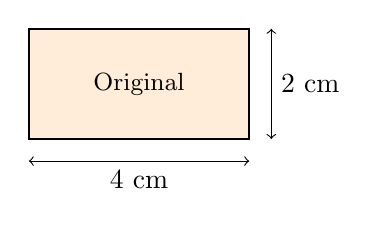
\begin{tikzpicture}[scale=0.7]
  \draw[thick,fill=orange!15] (0,0) rectangle (4,2);
  \draw[<->] (0,-0.4) -- (4,-0.4);
  \node[below] at (2,-0.4) {$4$ cm};
  \draw[<->] (4.4,0) -- (4.4,2);
  \node[right] at (4.4,1) {$2$ cm};
  \node at (2,1) {\small Original};
\end{tikzpicture}
\end{center}
\end{questionText}
\choiceA{$2$ cm by $1$ cm}
\choiceB{$4$ cm by $2$ cm}
\choiceC{$8$ cm by $4$ cm}
\choiceD{$20$ cm by $10$ cm}
\correctAnswer{C}
\explanation{Scale ratio: $\frac{10}{5} = 2$. New dimensions: $4 \times 2 = 8$ cm by $2 \times 2 = 4$ cm.}
\end{practiceQuestion}

\begin{practiceQuestion}{6-5-q22}{sa}
\begin{questionText}
Name two different cross-section shapes you can get from slicing a cube.
\end{questionText}
\correctAnswer{Any two of: square, rectangle, triangle, pentagon, hexagon}
\explanation{A cube can be sliced to produce squares, rectangles, triangles, pentagons, or hexagons depending on the angle and position of the cut.}
\end{practiceQuestion}

\begin{practiceQuestion}{6-6-q03}{mc}
\begin{questionText}
Two vertical angles are formed by intersecting lines. One angle is $72°$. What is the vertical angle?
\end{questionText}
\choiceA{$18°$}
\choiceB{$72°$}
\choiceC{$108°$}
\choiceD{$288°$}
\correctAnswer{B}
\explanation{Vertical angles are always equal. If one is $72°$, the vertical angle is also $72°$.}
\end{practiceQuestion}

\begin{practiceQuestion}{6-7-q06}{mc}
\begin{questionText}
Point $E(-4, -1)$ is translated left $3$ and up $5$. What are the coordinates of $E'$?
\end{questionText}
\choiceA{$(-7, 4)$}
\choiceB{$(-1, -6)$}
\choiceC{$(-1, 4)$}
\choiceD{$(-7, -6)$}
\correctAnswer{A}
\explanation{Left $3$: $-4 - 3 = -7$. Up $5$: $-1 + 5 = 4$. So $E'(-7, 4)$.}
\end{practiceQuestion}

\begin{practiceQuestion}{6-8-q15}{mc}
\begin{questionText}
A model of a building uses scale $1:200$. The model is $0.3$ m tall. How tall is the real building?
\end{questionText}
\choiceA{$6$ m}
\choiceB{$30$ m}
\choiceC{$60$ m}
\choiceD{$600$ m}
\correctAnswer{C}
\explanation{$0.3 \times 200 = 60$ m.}
\end{practiceQuestion}

\begin{practiceQuestion}{7-4-q21}{sa}
\begin{questionText}
A figure is made of a semicircle with diameter $10$ cm and a rectangle $10$ cm by $6$ cm. What is the total area? Use $\pi \approx 3.14$.
\end{questionText}
\correctAnswer{$99.25$ cm$^2$}
\explanation{Rectangle: $10 \times 6 = 60$ cm$^2$. Semicircle: $\frac{1}{2} \times 3.14 \times 5^2 = \frac{1}{2} \times 78.5 = 39.25$ cm$^2$. Total: $60 + 39.25 = 99.25$ cm$^2$.}
\end{practiceQuestion}

\begin{practiceQuestion}{7-5-q24}{sa}
\begin{questionText}
A triangular prism has a right-triangle base with legs $3$ cm and $4$ cm. The prism is $12$ cm long. The hypotenuse of the triangle is $5$ cm. What is the total surface area?
\end{questionText}
\correctAnswer{$156$ cm$^2$}
\explanation{Two triangles: $2 \times \frac{1}{2} \times 3 \times 4 = 12$ cm$^2$. Three rectangles: $3 \times 12 + 4 \times 12 + 5 \times 12 = 36 + 48 + 60 = 144$ cm$^2$. Total: $12 + 144 = 156$ cm$^2$.}
\end{practiceQuestion}

\begin{practiceQuestion}{7-6-q13}{mc}
\begin{questionText}
If you triple the height of a rectangular prism while keeping the base the same, what happens to the volume?
\end{questionText}
\choiceA{It stays the same}
\choiceB{It doubles}
\choiceC{It triples}
\choiceD{It increases by a factor of $9$}
\correctAnswer{C}
\explanation{$V = Bh$. If $h$ becomes $3h$, then $V = B(3h) = 3Bh$. The volume triples.}
\end{practiceQuestion}

\begin{practiceQuestion}{7-7-q01}{mc}
\begin{questionText}
What is the volume of a cylinder with radius $3$ cm and height $10$ cm? Use $\pi \approx 3.14$.
\end{questionText}
\choiceA{$30$ cm$^3$}
\choiceB{$94.2$ cm$^3$}
\choiceC{$282.6$ cm$^3$}
\choiceD{$565.2$ cm$^3$}
\correctAnswer{C}
\explanation{$V = \pi r^2 h = 3.14 \times 9 \times 10 = 282.6$ cm$^3$.}
\end{practiceQuestion}

\begin{practiceQuestion}{8-1-q04}{mc}
\begin{questionText}
A company wants to know if customers like a new product. They survey only customers who bought the product last week. What is the problem with this sample?
\end{questionText}
\choiceA{The sample is too large}
\choiceB{The sample is biased toward recent buyers}
\choiceC{The sample is random}
\choiceD{There is no problem}
\correctAnswer{B}
\explanation{Only surveying recent buyers introduces bias — they may feel differently than all customers.}
\end{practiceQuestion}

\begin{practiceQuestion}{8-3-q14}{mc}
\begin{questionText}
If the difference between two group means is more than $2$ times the MAD, the difference is generally considered:
\end{questionText}
\choiceA{Not meaningful}
\choiceB{Meaningless}
\choiceC{Meaningful}
\choiceD{Impossible to determine}
\correctAnswer{C}
\explanation{When the difference between means is more than $2$ MADs, there is little overlap and the difference is considered meaningful.}
\end{practiceQuestion}

\begin{practiceQuestion}{8-4-q10}{mc}
\begin{questionText}
Group A: median $55$, IQR $10$. Group B: median $55$, IQR $25$. What can you conclude?
\end{questionText}
\choiceA{Group A has a higher center}
\choiceB{Group B has a higher center}
\choiceC{Both groups have the same center, but Group B is more variable}
\choiceD{Both groups are identical}
\correctAnswer{C}
\explanation{Same median ($55$), but Group B's larger IQR ($25$ vs.\ $10$) means its data is more spread out.}
\end{practiceQuestion}

\begin{practiceQuestion}{8-5-q04}{mc}
\begin{questionText}
Data: $12, 15, 21, 23, 27, 30, 35$. In a stem-and-leaf plot, what are the stems?
\end{questionText}
\choiceA{$1, 2, 3$}
\choiceB{$2, 5, 1, 3, 7, 0, 5$}
\choiceC{$12, 15, 21, 23, 27, 30, 35$}
\choiceD{$10, 20, 30$}
\correctAnswer{A}
\explanation{The stems are the tens digits: $1$ (for $12, 15$), $2$ (for $21, 23, 27$), $3$ (for $30, 35$).}
\end{practiceQuestion}

\begin{practiceQuestion}{9-3-q29}{gsa}
\begin{questionText}
The table shows the results of drawing marbles from a bag $50$ times (with replacement). Based on the data, what is the experimental probability of drawing a green marble? Write your answer as a decimal.

\begin{center}
\begin{tabular}{|c|c|}
\hline
\textbf{Color} & \textbf{Times Drawn} \\
\hline
Red & $18$ \\
\hline
Green & $12$ \\
\hline
Blue & $20$ \\
\hline
\end{tabular}
\end{center}
\end{questionText}
\correctAnswer{$0.24$}
\explanation{$P = \frac{12}{50} = 0.24$.}
\end{practiceQuestion}

\begin{practiceQuestion}{9-6-q22}{sa}
\begin{questionText}
Two dice are rolled. What is the probability that the sum is exactly $6$? Write your answer as a fraction in simplest form.
\end{questionText}
\correctAnswer{$\frac{5}{36}$}
\explanation{Outcomes with sum $6$: $(1,5), (2,4), (3,3), (4,2), (5,1)$ — $5$ out of $36$. $P = \frac{5}{36}$.}
\end{practiceQuestion}

\begin{practiceQuestion}{9-7-q08}{mc}
\begin{questionText}
In a simulation, you roll a die $120$ times to model rolling a $5$. About how many times do you expect to roll a $5$?
\end{questionText}
\choiceA{$5$}
\choiceB{$12$}
\choiceC{$20$}
\choiceD{$60$}
\correctAnswer{C}
\explanation{$P(5) = \frac{1}{6}$. Expected: $120 \times \frac{1}{6} = 20$.}
\end{practiceQuestion}
